% =========================================================================
%  PÓSTER — Vulnerabilidad de la red vial primaria de carga de Colombia
%  Tamaño A0 vertical (841 x 1189 mm). Para otro tamaño, cambie el
%  paperwidth/paperheight y las coordenadas (están en mm, medidas desde
%  arriba con \arriba{...}).
%  Compilar desde esta carpeta:  latexmk -pdf poster.tex
%  Las cifras salen de outputs/resultados/ (cierres_aristas.csv,
%  intermediacion_y_carga.csv, validacion.txt) y el mapa de
%  outputs/figuras/mapa_poster.png (scripts/08_figuras.py).
% =========================================================================
\documentclass{article}
\usepackage[paperwidth=841mm, paperheight=1189mm, margin=0mm]{geometry}
\usepackage[T1]{fontenc}
\usepackage[scaled]{helvet}
\renewcommand{\familydefault}{\sfdefault}
\usepackage{graphicx}
\usepackage{tikz}
\usetikzlibrary{calc}
\graphicspath{{../../outputs/figuras/}}
\pagestyle{empty}

% ---------------------------------------------------------------- colores
\definecolor{fondo}{HTML}{F7F6F2}
\definecolor{noche}{HTML}{1F3A5F}
\definecolor{tinta}{HTML}{2B2B29}
\definecolor{suave}{HTML}{6B6A65}
\definecolor{azul}{HTML}{2A78D6}
\definecolor{naranja}{HTML}{EB6834}
\definecolor{aqua}{HTML}{1BAF7A}
\definecolor{gris}{HTML}{9A9993}
\definecolor{grisclaro}{HTML}{D9D8D3}
\definecolor{rojo}{HTML}{E34948}

% ---------------------------------------------------------------- letra
% Los nodos de TikZ con ancho fijo dejan el espacio entre palabras al tamaño de la letra
% normal: \spaceskip=0pt devuelve el espacio propio del nuevo tamaño, \rightskip deja el
% borde derecho libre (sin justificar) y el \hyphenpenalty evita partir palabras. Cada
% texto de varias líneas termina en \par, para que TikZ corte las líneas con estos ajustes.
\newcommand{\letra}[2]{\fontsize{#1}{#2}\selectfont\spaceskip=0pt\xspaceskip=0pt%
  \rightskip=0pt plus 1fil\hyphenpenalty=10000\exhyphenpenalty=10000\relax}
\newcommand{\arriba}[1]{{1189-(#1)}}          % y medido desde el borde de arriba
\newcommand{\titulo}[1]{{\letra{48}{56}\bfseries\color{noche}#1}}
\newcommand{\cuerpo}{\letra{31}{39}}

\begin{document}
\noindent
\begin{tikzpicture}[x=1mm, y=1mm]
% fondo y encabezado
\fill[fondo] (0,0) rectangle (841,1189);
\fill[noche] (0,\arriba{0}) rectangle (841,\arriba{215});
\fill[naranja] (0,\arriba{215}) rectangle (841,\arriba{221});

\node[anchor=north west, text width=770mm, text=white] at (40,\arriba{28})
  {\letra{100}{112}\bfseries ¿Qué carretera de Colombia nos cuesta más cuando se cierra?\par};
\node[anchor=north west, text width=770mm, text=white] at (40,\arriba{150})
  {\letra{34}{42}Evaluación de la vulnerabilidad de la red vial primaria de carga de Colombia
   mediante teoría de grafos\par};
\node[anchor=north west, text=grisclaro] at (40,\arriba{186})
  {\letra{28}{34}David Catral \textperiodcentered{} Gabriel Salcedo \textperiodcentered{} Isaac Suárez
   \qquad Teoría de Grafos \textperiodcentered{} Universidad del Rosario \textperiodcentered{} 2026-II};

% ---------------------------------------------------------------- 3 cifras
\foreach \x/\tono/\cifra/\texto in {
  40/naranja/{9,45}/{millones de toneladas al año se quedan \textbf{sin salida} si se cierra
     Buenaventura--Dagua, la única vía del mayor puerto del Pacífico.},
  302/azul/{908.600}/{millones de pesos al año cuesta cerrar \textbf{Buga--Zarzal} (Valle).
     Dos semanas cerrada: 34.800 millones.},
  564/noche/{18}/{carreteras son \textbf{críticas}: mueven mucha carga y, si se cierran,
     el único desvío es largo y caro.}} {
  \fill[white] (\x,\arriba{240}) rectangle ++(237,-122);
  \fill[\tono] (\x,\arriba{240}) rectangle ++(237,-7);
  \node[anchor=north west, text=\tono] at (\x+10,\arriba{252})
    {\letra{108}{108}\bfseries\cifra};
  \node[anchor=north west, text width=217mm, text=tinta] at (\x+10,\arriba{297})
    {\letra{27}{34}\texto\par};
}

% ---------------------------------------------------------------- columna izquierda
% El problema
\node[anchor=north west] at (40,\arriba{385}) {\titulo{El problema}};
\node[anchor=north west, text width=360mm, text=tinta] at (40,\arriba{410})
  {\cuerpo Casi toda la carga del país viaja en camión por unas pocas carreteras. Cuando
   un derrumbe, un bloqueo o una obra cierra una de ellas, los camiones dan la vuelta por
   un camino más largo y más caro, o se quedan sin camino.\par\vspace{3mm}
   \textbf{¿Cuáles cierres hacen más daño?}\par};

% Qué es un grafo + ejemplo real
\node[anchor=north west] at (40,\arriba{510}) {\titulo{La herramienta: un grafo}};
\node[anchor=north west, text width=360mm, text=tinta] at (40,\arriba{535})
  {\cuerpo Un mapa simplificado: \textbf{puntos} (25 ciudades y 28 cruces) unidos por
   \textbf{líneas} (77 carreteras). Cada línea tiene un \textbf{peso}: lo que cuesta llevar
   una tonelada por ella. Así el computador halla la ruta más barata y, si una vía se
   cierra, el mejor desvío.\par};

% mini grafo: el caso Buenaventura -> Bogotá
\coordinate (bv) at (55,\arriba{660});
\coordinate (da) at (105,\arriba{660});
\coordinate (bu) at (165,\arriba{632});
\coordinate (za) at (240,\arriba{632});
\coordinate (bo) at (370,\arriba{655});
\coordinate (ca) at (165,\arriba{692});
\coordinate (ne) at (270,\arriba{692});
\draw[azul, line width=2.2mm] (bv)--(da)--(bu)--(za)--(bo);
\draw[naranja, line width=1.6mm, dash pattern=on 5mm off 3mm] (da)--(ca)--(ne)--(bo);
\node[text=rojo] at ($(bu)!0.5!(za)$) {\letra{80}{80}\bfseries ×};
\foreach \p in {bv,da,bu,za,bo,ca,ne} \fill[tinta] (\p) circle (3.2mm);
\node[anchor=north, text=tinta] at ([yshift=-5mm]bv) {\letra{21}{25}Buenaventura};
\node[anchor=south, text=tinta] at ([yshift=5mm]da) {\letra{21}{25}Dagua};
\node[anchor=south, text=tinta] at ([yshift=5mm]bu) {\letra{21}{25}Buga};
\node[anchor=south, text=tinta] at ([yshift=5mm]za) {\letra{21}{25}Zarzal};
\node[anchor=south, text=tinta] at ([yshift=5mm]bo) {\letra{21}{25}\bfseries Bogotá};
\node[anchor=north, text=tinta] at ([yshift=-5mm]ca) {\letra{21}{25}Cali};
\node[anchor=north, text=tinta] at ([yshift=-5mm]ne) {\letra{21}{25}Neiva};
\draw[azul, line width=2.2mm] (42,\arriba{724}) -- ++(16,0);
\node[anchor=west, text=tinta] at (62,\arriba{724})
  {\letra{23}{28}Ruta normal Buenaventura--Bogotá: \textbf{470 km}};
\draw[naranja, line width=1.6mm, dash pattern=on 5mm off 3mm] (42,\arriba{738}) -- ++(16,0);
\node[anchor=west, text=tinta] at (62,\arriba{738})
  {\letra{23}{28}Con Buga--Zarzal cerrada ({\color{rojo}\textbf{×}}): \textbf{821 km},
   87.106 pesos más por tonelada};

% Lo que más cuesta cerrar
\node[anchor=north west] at (40,\arriba{768}) {\titulo{Las vías más caras de cerrar}};
\node[anchor=north west, text=suave] at (40,\arriba{790})
  {\letra{21}{25}Miles de millones de pesos al año, con desvío disponible};
\foreach \i/\nombre/\v/\cifra in {0/Buga -- Zarzal/908.6/{908,6},
                                  1/El Guamo -- El Carmen de Bolívar/687.3/{687,3},
                                  2/Bosconia -- Aguachica/473.0/{473,0},
                                  3/Ibagué -- Zarzal/383.9/{383,9},
                                  4/Bogotá -- Tocancipá/327.2/{327,2}} {
  \pgfmathsetmacro{\y}{1189-810-\i*15}
  \pgfmathsetmacro{\largo}{\v/908.6*140}
  \ifnum\i=0 \def\col{azul}\else \def\col{gris}\fi
  \node[anchor=east, text=tinta] at (200,\y-4.5) {\letra{21}{25}\nombre};
  \fill[\col] (204,\y) rectangle ++(\largo,-9);
  \node[anchor=west, text=tinta] at (204+\largo+2,\y-4.5) {\letra{21}{25}\bfseries\cifra};
}

% ---------------------------------------------------------------- columna derecha: mapa
\node[anchor=north west] at (430,\arriba{385}) {\titulo{Dónde están las vías críticas}};
\foreach \fila/\col/\x/\ancho/\texto in {
  0/naranja/430/2.2/{Crítica: mucha carga y mal desvío},
  0/azul/625/1.2/{Mucha carga, buen desvío},
  1/aqua/430/1.2/{Poca carga, mal desvío},
  1/gris/625/1.2/{Poca carga, buen desvío}} {
  \pgfmathsetmacro{\y}{1189-420-\fila*14}
  \draw[\col, line width=\ancho mm] (\x,\y) -- ++(14,0);
  \node[anchor=west, text=tinta] at (\x+17,\y) {\letra{21}{25}\texto};
}
\node[anchor=north west, inner sep=0pt] at (430,\arriba{448})
  {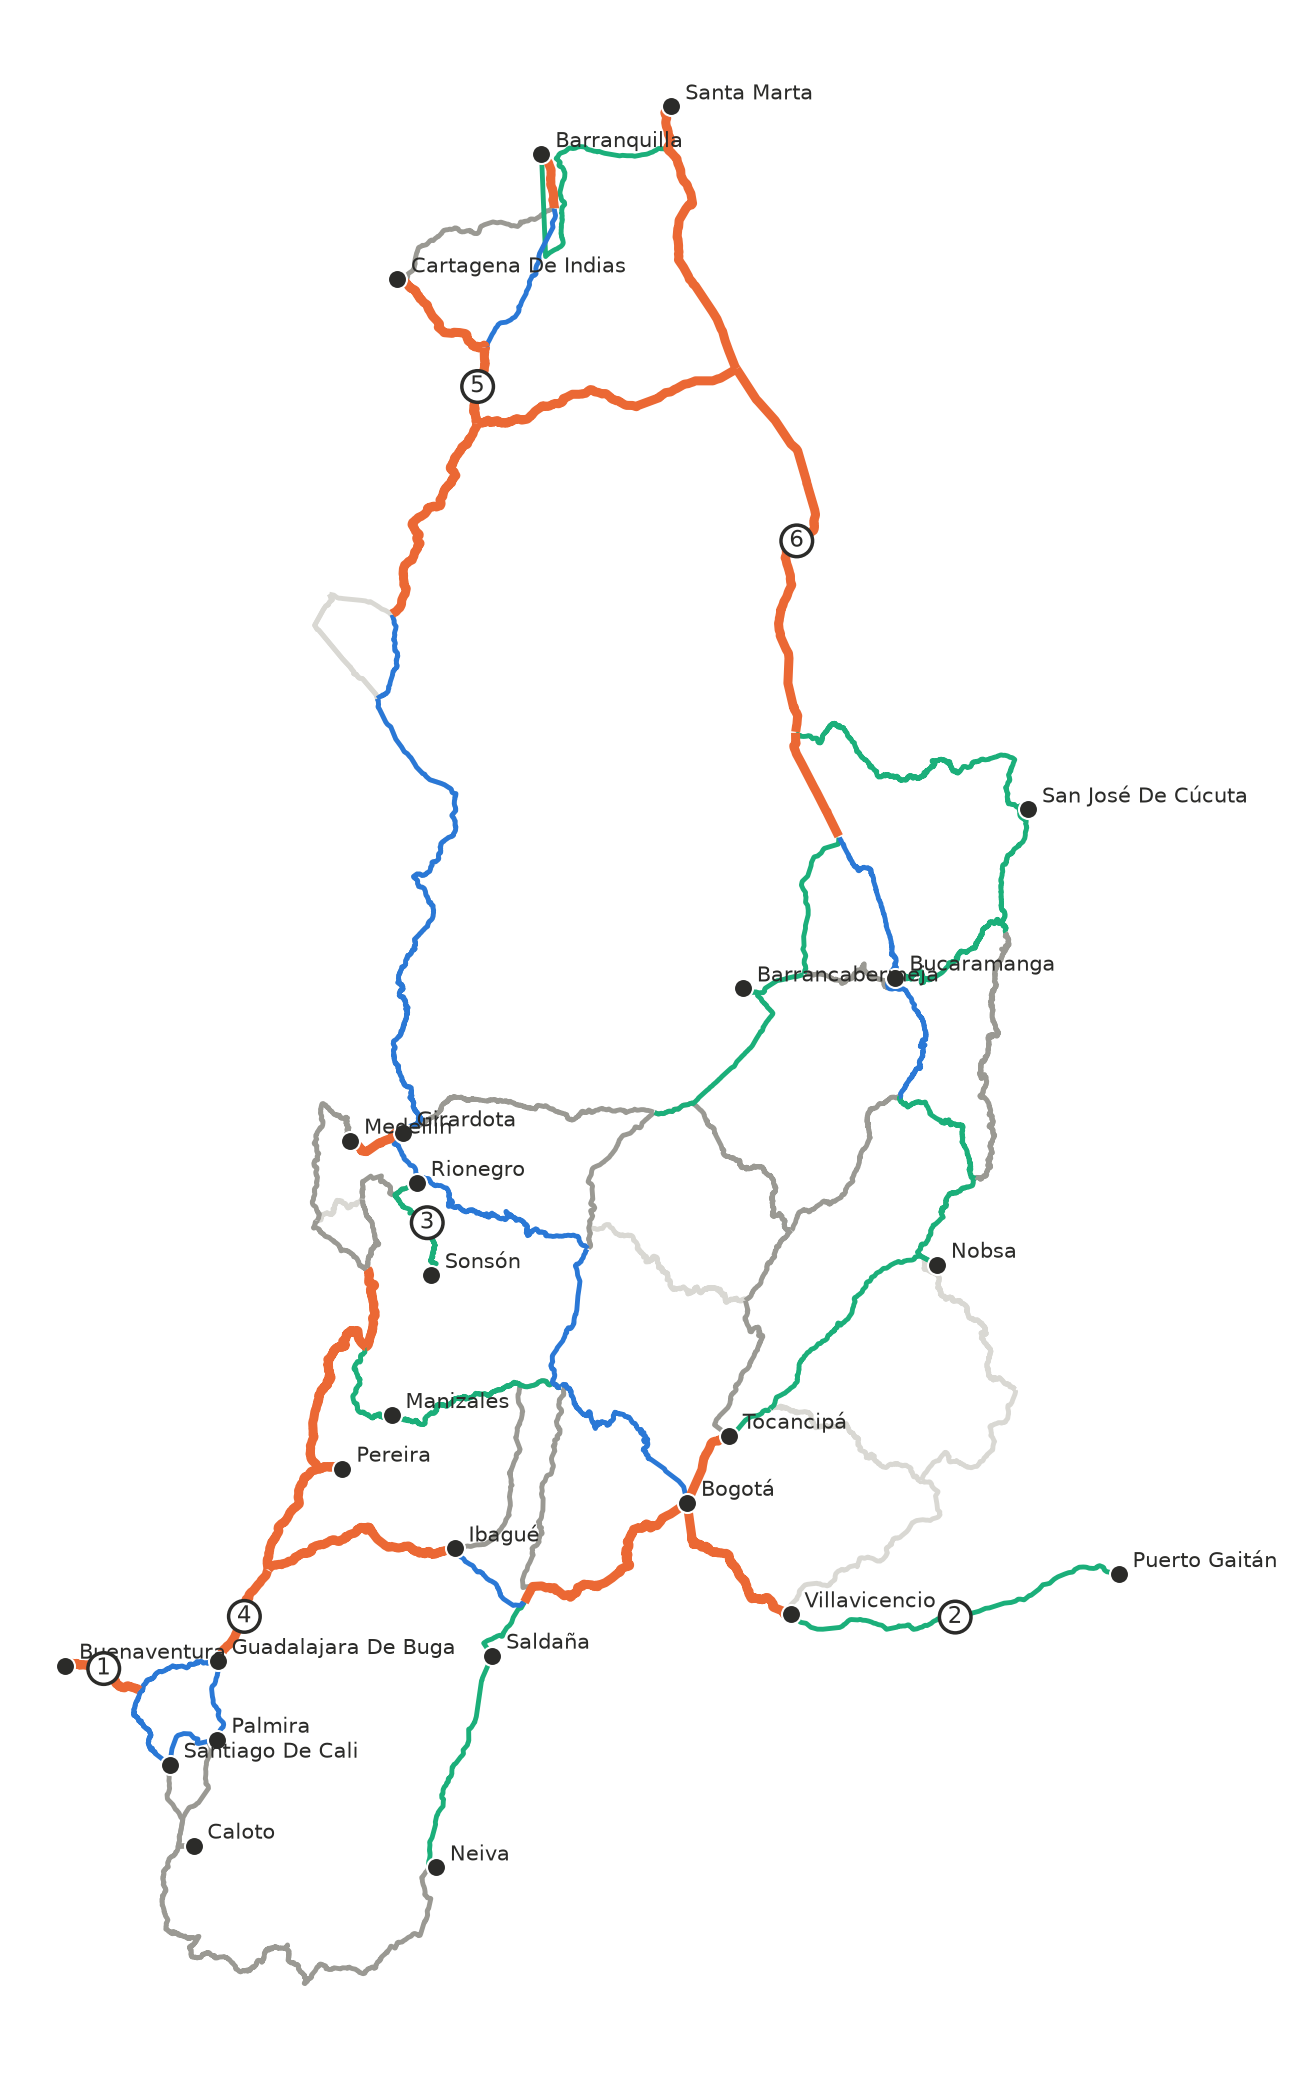
\includegraphics[height=425mm]{mapa_poster.png}};

% los seis cierres más graves, al lado del mapa
\node[anchor=north west, text width=105mm, text=noche] at (700,\arriba{452})
  {\letra{25}{30}\bfseries Los 6 cierres más graves\par};
\foreach \n/\y/\via/\dano/\tono in {
  1/488/{Buenaventura -- Dagua}/{9,45 millones de t sin salida}/naranja,
  2/540/{Villavicencio -- Puerto Gaitán}/{0,98 millones de t sin salida}/aqua,
  3/592/{Sonsón -- Rionegro}/{0,97 millones de t sin salida}/aqua,
  4/644/{Buga -- Zarzal}/{908.600 millones al año}/naranja,
  5/696/{El Guamo -- El Carmen de Bolívar}/{687.300 millones al año}/naranja,
  6/748/{Bosconia -- Aguachica}/{473.000 millones al año}/naranja} {
  \draw[tinta, line width=0.5mm, fill=white] (707,\arriba{\y}) circle (6.5mm);
  \node[text=tinta] at (707,\arriba{\y}) {\letra{22}{22}\bfseries\n};
  \node[anchor=north west, text width=85mm, text=tinta] at (717,\arriba{\y-6})
    {\letra{21}{25}\textbf{\via}\par\vspace{1mm}{\color{\tono}\letra{20}{24}\dano}\par};
}
\node[anchor=north west, text width=105mm, text=suave] at (700,\arriba{800})
  {\letra{19}{24}1--3 dejan una ciudad aislada. 4--6 obligan a los desvíos más caros.\par};

% ---------------------------------------------------------------- cómo lo hicimos
\node[anchor=north west] at (40,\arriba{905}) {\titulo{Cómo lo hicimos}};
\foreach \n/\x/\cab/\texto in {
  1/40/Datos/{Mapa oficial de carreteras (INVIAS) y casi 6 millones de viajes de camión de 2015 (RNDC).},
  2/235/Del mapa al grafo/{Limpiamos el mapa y lo resumimos en 25 ciudades, 28 cruces y 77 carreteras.},
  3/430/Ruta más barata/{Cada tonelada viaja por el camino más barato entre su origen y su destino.},
  4/625/Cerrar y medir/{Cerramos cada carretera, una por una, y medimos cuánto más se paga o cuánta carga queda sin salida.}} {
  \fill[white] (\x,\arriba{932}) rectangle ++(176,-104);
  \fill[noche] (\x+18,\arriba{952}) circle (10mm);
  \node[text=white] at (\x+18,\arriba{952}) {\letra{34}{34}\bfseries\n};
  \node[anchor=west, text=noche, text width=135mm] at (\x+33,\arriba{952})
    {\letra{27}{31}\bfseries\cab\par};
  \node[anchor=north west, text width=158mm, text=tinta] at (\x+9,\arriba{970})
    {\letra{23}{29}\texto\par};
}

% ---------------------------------------------------------------- la lección
\fill[noche] (0,\arriba{1055}) rectangle (841,\arriba{1152});
\node[anchor=north west, text width=410mm, text=white] at (40,\arriba{1068})
  {\letra{42}{48}\bfseries Mirar solo el mapa no basta.\par\vspace{3mm}
   \letra{23}{29}\mdseries Una vía puede parecer secundaria y mover muchísima carga
   (Buenaventura--Dagua), o estar en el centro de todo y tener un buen desvío (Puerto
   Triunfo--Honda). Lo que hace crítica a una carretera es \textbf{cuánta carga mueve} y
   \textbf{qué tan malo es su desvío}.\par};
\node[anchor=north west, text width=320mm, text=white] at (480,\arriba{1068})
  {\letra{32}{38}\bfseries ¿Para qué sirve?\par\vspace{2mm}
   \letra{23}{30}\mdseries
   \textbullet\; Saber dónde invertir primero en mantenimiento.\par
   \textbullet\; Planear desvíos antes de que ocurra un cierre.\par
   \textbullet\; Calcular en pesos cuánto cuesta un derrumbe, con una herramienta interactiva.\par};

% ---------------------------------------------------------------- pie
\node[anchor=north west, text width=780mm, text=suave] at (40,\arriba{1160})
  {\letra{17}{21}Datos: red vial INVIAS (HDX \emph{Colombia: Roads}), Registro Nacional de Despachos
   de Carga 2015 (Ministerio de Transporte), DIVIPOLA (DANE). Pesos de 2015. Las cifras son un
   mínimo: no incluyen congestión ni vías secundarias. Código y datos:
   github.com/gabrielsalcedo/graph-theory\par};
\end{tikzpicture}
\end{document}
